\documentclass[oneside]{book}
\usepackage{lmodern}
\usepackage{amssymb,amsmath}
\usepackage{ifxetex,ifluatex}
\usepackage{fixltx2e} % provides \textsubscript
\ifnum 0\ifxetex 1\fi\ifluatex 1\fi=0 % if pdftex
  \usepackage[T1]{fontenc}
  \usepackage[utf8]{inputenc}
\else % if luatex or xelatex
  \ifxetex
    \usepackage{mathspec}
  \else
    \usepackage{fontspec}
  \fi
  \defaultfontfeatures{Ligatures=TeX,Scale=MatchLowercase}
\fi
% use upquote if available, for straight quotes in verbatim environments
\IfFileExists{upquote.sty}{\usepackage{upquote}}{}
% use microtype if available
\IfFileExists{microtype.sty}{%
\usepackage[]{microtype}
\UseMicrotypeSet[protrusion]{basicmath} % disable protrusion for tt fonts
}{}
\PassOptionsToPackage{hyphens}{url} % url is loaded by hyperref
\usepackage[unicode=true]{hyperref}
\hypersetup{
            pdftitle={Vegetation modelling},
            pdfauthor={Hans Verbeeck, Elizabeth Kearsley, Félicien Meunier, Marc Peaucelle},
            pdfborder={0 0 0},
            breaklinks=true}
\urlstyle{same}  % don't use monospace font for urls
\usepackage[left=3cm,right=3cm,top=2cm,bottom=2cm]{geometry}
\usepackage{natbib}
\bibliographystyle{apalike}
\usepackage{longtable,booktabs}
% Fix footnotes in tables (requires footnote package)
\IfFileExists{footnote.sty}{\usepackage{footnote}\makesavenoteenv{long table}}{}
\usepackage{graphicx,grffile}
\makeatletter
\def\maxwidth{\ifdim\Gin@nat@width>\linewidth\linewidth\else\Gin@nat@width\fi}
\def\maxheight{\ifdim\Gin@nat@height>\textheight\textheight\else\Gin@nat@height\fi}
\makeatother
% Scale images if necessary, so that they will not overflow the page
% margins by default, and it is still possible to overwrite the defaults
% using explicit options in \includegraphics[width, height, ...]{}
\setkeys{Gin}{width=\maxwidth,height=\maxheight,keepaspectratio}
\IfFileExists{parskip.sty}{%
\usepackage{parskip}
}{% else
\setlength{\parindent}{0pt}
\setlength{\parskip}{6pt plus 2pt minus 1pt}
}
\setlength{\emergencystretch}{3em}  % prevent overfull lines
\providecommand{\tightlist}{%
  \setlength{\itemsep}{0pt}\setlength{\parskip}{0pt}}
\setcounter{secnumdepth}{5}
% Redefines (sub)paragraphs to behave more like sections
\ifx\paragraph\undefined\else
\let\oldparagraph\paragraph
\renewcommand{\paragraph}[1]{\oldparagraph{#1}\mbox{}}
\fi
\ifx\subparagraph\undefined\else
\let\oldsubparagraph\subparagraph
\renewcommand{\subparagraph}[1]{\oldsubparagraph{#1}\mbox{}}
\fi

% set default figure placement to htbp
\makeatletter
\def\fps@figure{htbp}
\makeatother

\usepackage{booktabs}
\usepackage{fancyhdr}

\AtBeginDocument{\let\maketitle\relax} % To relax 

% Remove page number on page parts
\usepackage{etoolbox}
\patchcmd{\part}{\thispagestyle{plain}}{\thispagestyle{empty}}{}{}

% Header and font 
\usepackage{fancyhdr}
\pagestyle{fancy}
\fancyhf{} % sets both header and footer to nothing
\renewcommand{\headrulewidth}{0pt} % Remove line

\fancyhead[L,C,R]{} % Empty header
\fancyfoot[C]{\thepage} % Footer, center, page number
\fancyfoot[L,R]{} % Empty footer on left and right

\title{Vegetation modelling}
\author{Hans Verbeeck, Elizabeth Kearsley, Félicien Meunier, Marc Peaucelle}
\date{2020-05-27}

\begin{document}
\maketitle

\newcommand{\plogo}{\fbox{$\mathcal{PL}$}} % Generic dummy publisher logo
\frontmatter


\begin{titlepage} % Suppresses headers and footers on the title page

	\centering % Centre everything on the title page
	
	\scshape % Use small caps for all text on the title page
	
	\vspace*{\baselineskip} % White space at the top of the page
	
	%------------------------------------------------
	%	Title
	%------------------------------------------------
	
	\vspace{8\baselineskip}
	
	\rule{\textwidth}{1.6pt}\vspace*{-\baselineskip}\vspace*{2pt} % Thick horizontal rule
	\rule{\textwidth}{0.4pt} % Thin horizontal rule
	
	\vspace{0.75\baselineskip} % Whitespace above the title
	
	{\LARGE Vegetation modelling\\} % Title
	
	\vspace{0.75\baselineskip} % Whitespace below the title
	
	\rule{\textwidth}{0.4pt}\vspace*{-\baselineskip}\vspace{3.2pt} % Thin horizontal rule
	\rule{\textwidth}{1.6pt} % Thick horizontal rule
	
	\vspace{2\baselineskip} % Whitespace after the title block
	
	%------------------------------------------------
	%	Subtitle
	%------------------------------------------------
	
	Course XXXX % Subtitle or further description
	
	\vspace*{3\baselineskip} % Whitespace under the subtitle
	
	%------------------------------------------------
	%	Editor(s)
	%------------------------------------------------
	
	Written By
	
	\vspace{0.5\baselineskip} % Whitespace before the editors
	
	{\scshape Hans Verbeeck, Elizabeth Kearsley, Felicien Meunier, Marc Peaucelle \\} % Editor list
	
	\vspace{0.5\baselineskip} % Whitespace below the editor list
	
	\textit{Ghent University \\} % Editor affiliation
	
	\vfill % Whitespace between editor names and publisher logo
	
	%------------------------------------------------
	%	Publisher
	%------------------------------------------------
	
	%\plogo % Publisher logo
	
	
\includegraphics[width=40mm]{figures/UGhent.png}
	
	\vspace{0.3\baselineskip} % Whitespace under the publisher logo
	
	2020 % Publication year
	
	%{\large publisher} % Publisher

\end{titlepage}

{
\setcounter{tocdepth}{1}
\tableofcontents
}
\mainmatter

\chapter{Introduction}\label{intro}

\section{Soil-Plant-Atmosphere continuum: the central role of
vegetation}\label{soil-plant-atmosphere-continuum-the-central-role-of-vegetation}

\section{Why do we need modelling?}\label{why-do-we-need-modelling}

\section{Components of a model}\label{components-of-a-model}

\section{The history of vegetation
models}\label{the-history-of-vegetation-models}

\subsection{Early history of vegetation
modelling}\label{early-history-of-vegetation-modelling}

\subsection{The first DVGMs centered around carbon
fluxes}\label{the-first-dvgms-centered-around-carbon-fluxes}

\subsection{A new generation of DGVMs centered around vegetation
functioning}\label{a-new-generation-of-dgvms-centered-around-vegetation-functioning}

\section{Model types}\label{model-types}

\section{Structure of the course}\label{structure-of-the-course}

\begin{figure}

{\centering 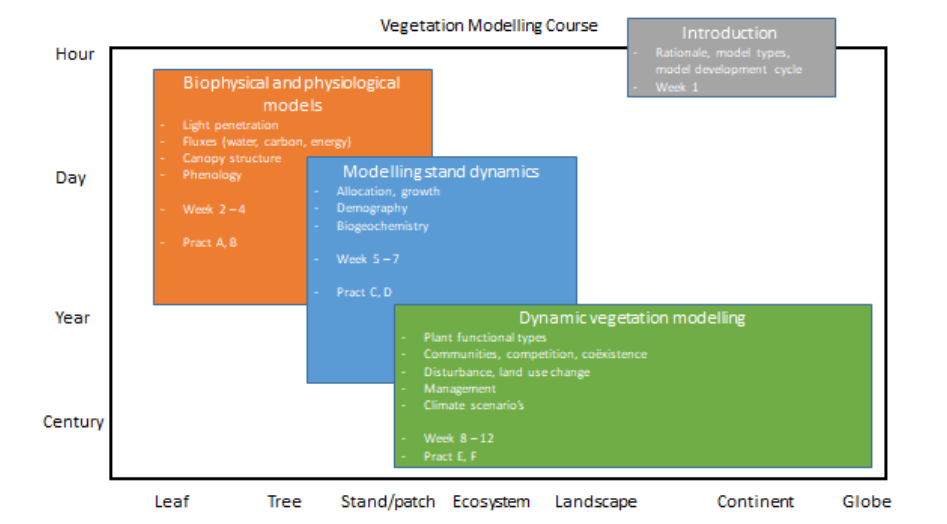
\includegraphics[width=0.8\linewidth]{figures/Figure_course} 

}

\caption{Here is the structure of the course!}\label{fig:nice-fig2}
\end{figure}

\part{Biophysical and physiological
models}\label{part-biophysical-and-physiological-models}

\chapter{Modelling plant basic
processes}\label{modelling-plant-basic-processes}

\chaptermark{photsynthesis}

\section{Photosynthesis and stomatal
models}\label{photosynthesis-and-stomatal-models}

\section{Respiration models}\label{respiration-models}

\section{Transpiration}\label{transpiration}

\section{Upscaling from leaf to
canopy}\label{upscaling-from-leaf-to-canopy}

\chapter{Modelling light penetration, vegetation canopy representation,
and energy
balance}\label{modelling-light-penetration-vegetation-canopy-representation-and-energy-balance}

\chaptermark{Light}

\section{Representing canopy structure in
models}\label{representing-canopy-structure-in-models}

\section{Direct and diffuse light}\label{direct-and-diffuse-light}

\section{Ecosystem energy balance}\label{ecosystem-energy-balance}

\chapter{Temporal and seasonal
dynamics}\label{temporal-and-seasonal-dynamics}

\chaptermark{dynamics}

\section{Leaf phenology}\label{leaf-phenology}

\section{Drivers of seasonality and
phenology}\label{drivers-of-seasonality-and-phenology}

\part{Modelling vegetation
dynamics}\label{part-modelling-vegetation-dynamics}

\chapter{Modelling growth, timber production and Carbon
allocation}\label{modelling-growth-timber-production-and-carbon-allocation}

\chaptermark{Growth}

\section{Empirical growth modelling: growth
curves}\label{empirical-growth-modelling-growth-curves}

\section{Process-based growth modelling: C-allocation
models}\label{process-based-growth-modelling-c-allocation-models}

\chapter{Modelling vegetation dynamics and
demography}\label{modelling-vegetation-dynamics-and-demography}

\chaptermark{Dynamics}

\section{Seed dispersal and
recruitment}\label{seed-dispersal-and-recruitment}

\section{Mortality}\label{mortality}

\section{Gap models, individual and cohort based
models}\label{gap-models-individual-and-cohort-based-models}

\chapter{Modelling biogeochemical cycles in
vegetation}\label{modelling-biogeochemical-cycles-in-vegetation}

\chaptermark{Biogeochemical}

\section{Carbon cycle models: stocks and
fluxes}\label{carbon-cycle-models-stocks-and-fluxes}

\section{Nutrient cycle models: soil biogeochemical
models}\label{nutrient-cycle-models-soil-biogeochemical-models}

\section{Water balance}\label{water-balance}

\part{Upscaling and
applications}\label{part-upscaling-and-applications}

\chapter{Representing biodiversity in vegetation
models}\label{representing-biodiversity-in-vegetation-models}

\chaptermark{Biodiversity}

\section{Functional diversity}\label{functional-diversity}

\section{Competition models}\label{competition-models}

\section{Communities}\label{communities}

\chapter{Spatial heterogeneity, landscape scale,
metapopulations}\label{spatial-heterogeneity-landscape-scale-metapopulations}

\chaptermark{Heterogeneity}

\section{Patch dynamics}\label{patch-dynamics}

\section{Land-use changes}\label{land-use-changes}

\section{Fire and disturbance}\label{fire-and-disturbance}

\chapter{Upscaling from leaf/tree to
globe}\label{upscaling-from-leaftree-to-globe}

\chaptermark{Globe}

\section{Land surface models}\label{land-surface-models}

\section{DVGMs as a part of Earth system
models}\label{dvgms-as-a-part-of-earth-system-models}

\chapter{Model projections and scenario
analysis}\label{model-projections-and-scenario-analysis}

\chaptermark{Projections}

\section{Climate scenarios}\label{climate-scenarios}

\section{Land-use scenarios}\label{land-use-scenarios}

\section{Management scenarios}\label{management-scenarios}

\part{Practicals}\label{part-practicals}

\chapter*{Supporting material}\label{supporting-material}
\addcontentsline{toc}{chapter}{Supporting material}

Crash course, basic programming (R), theory about model evaluation etc.

\chapter*{Practical A}\label{practical-a}
\addcontentsline{toc}{chapter}{Practical A}

PC-room, supervised exercise

Simple model on diurnal variation in solar angle, radiation extinction
and photosynthesis in vegetation types with different and canopy
structure and LAI: grassland, broadleaved forest, coniferous forest

Scale: aggregated stand level (big leaf model)

Methodological focus: model formulation: translating a few equations
into code

Methodological focus: compiling code, running model, reading
input-output

\chapter*{Practical B}\label{practical-b}
\addcontentsline{toc}{chapter}{Practical B}

Group work, report, PC room

Modelling diurnal cycle of carbon and water fluxes for flux tower sites
(Savanna's Sahel)

Scale: aggregated stand level

Methodological focus: model-data comparison (goodness-of-fit), simple
parameter optimisation

\chapter*{Practical C}\label{practical-c}
\addcontentsline{toc}{chapter}{Practical C}

PC-room, supervised exercise

Modelling the size structure of a temperate forest (stand diameter
distribution)

Scale: forest stand

Methodological focus: initial conditions

\chapter*{Practical D}\label{practical-d}
\addcontentsline{toc}{chapter}{Practical D}

Group work, report, PC room

Modelling carbon stocks (above and belowground) and fluxes

Scale: ecosystem

Methodological focus: Spinup and sensitivity analysis (testing which
climate variables have strongest impact on stocks)

\chapter*{Practical E}\label{practical-e}
\addcontentsline{toc}{chapter}{Practical E}

PC-room, supervised exercise

Simulating forest succession, meta-analysis of trait dataset to
prescribe vegetation functional composition (using PEcAn-framework)

Scale: landscape

Methodological focus: parameter meta-analysis (PFT construction), data
assimilation

\chapter*{Practical F}\label{practical-f}
\addcontentsline{toc}{chapter}{Practical F}

PC-room, group work, microteaching

Climate/land use/management scenario analysis

Scale: site/globe? (Pecan framework) each group choses a question and a
model

Methodological focus: sensitivity and uncertainty analysis

\bibliography{book.bib,packages.bib}

\end{document}
